\section{Лекция 5 -- 2024-03-22}

\begin{definition}
  Однородная марковская цепь называется эргодичной, если $\exists \lim_{t\to\infty} p_{ij}(t) = \pi_j$
  (и $\pi_j \geqslant 0$, $\sum \pi_j = 1$).
\end{definition}

\begin{theorem}
  Если $\mathcal{S} = \left\{ S_1, S_2, \dots, S_m, \dots \right\}$,
  $\exists S_{j_0} \, \exists h>0 \exists \delta \in (0;1] \forall i :
    p_{i j_0}(h) \geqslant \delta$, тогда
    \begin{equation}\label{ergodi-eq-1}\tag{\ast}
      \exists \lim_{t\to\infty} p_{ij}(t) = \pi_j, \quad
      |p_{ij}(t) - \pi_j| \leslant (1-\delta)^{ \left[ \dfrac{t}{h} \right]  }
    \end{equation}
    .
\end{theorem}

\begin{corollary}
  \begin{enumerate}
    \item Из уравнения \eqref{ergodi-eq-1} следует, что для любого вектора
      начальных вероятностей:
      \[
        \exists \lim_{t\to\infty} p_j(t) = \pi_j,
        |p_j(t) - \pi_j| \leqslant (1-\delta)^{ \left[ \dfrac{t}{h} \right]   }
      \]
    
    \item В условиях теоремы, $\pi_j = \sum_{i} p_{ij}(t) \pi_i \leftrightarrow$ $\pi$ является
      собственным вектором $P(t)^T$, соответствующем $\lambda = 1$, но с оговоркой,
      что $\pi \neq 0$ (нулевой вектор не является собственным по определению).
      Эта система в векторной записи: $\pi = P(t)^T \pi$,
      \begin{proof}
        \[
          \pi_j = \lim_{s\to\infty} p_j(s+t) = \lim_{s\to\infty} \sum_i p_{ij}(t) p_t(s)
          \geqslant \lim_{s\to\infty} \sum_{i \leqslant N} p_{ij}(t) p_i(s)
          = \sum_{i \leqslant N} p_{ij}(t) \pi_i \Rightarrow \pi_j \geqslant \sum_i p_{ij}(t) \pi_i.
        \]
        \[
          \exists S_{j_1} : \pi_{j_1} > \sum_i p_{ij_1} \pi_i
        \]
        \[
          \sum_{j\leqslant N} = \lim_{t\to\infty} \sum_{j\leqslant N} p_{ij}(t) \leqslant 1.
        \]
        \[
          \sum_j \pi_j > \sum_j \sum_i p_{ij}(t) \pi_i = \sum_i \pi_i.
        \]
      \end{proof}

    \item \eqref{ergodi-eq-1} $\Rightarrow$ либо $\sum_j \pi_j = 1$ -- тогда это
      собственный вектор, либо $\sum_j \pi_j = 0$.

      \begin{proof}
        $\sum_j \pi_j \leqslant 1$ означает, что либо $\pi_j \pi_j = 1$, либо
        $\sum_j \pi_j < 1$. 
        $A = \sum_j \pi_j$ рассматривается
        $p(0) = \left( \dfrac{\pi_1}{A}, \dfrac{\pi_2}{A}, \dots \right)^T$.
        $\bar p(t)^T = p(0)^T \cdot P(t)$.
        \[
          p_j(t) = \sum_i p_i(0) p_{ij}(t) = \sum_i \dfrac{\pi_i}{A} p_{ij}(t)
          = \dfrac{\pi_j}{\sum_{k} \pi_k} = p_j(0)
          \Rightarrow
          \sum_j \pi_j = \sum_j p_j(0) = 1.
        \]
      \end{proof}
      
    \item В условиях теоремы: $\begin{cases} \bar{0} = \pi^T \cdot \Lambda, \\ \sum_j \pi_j = 1\end{cases}$
      Это условие можно получить из системы уравнений Колмогорова:
      $p'(t)^T = p(t)^T \cdot \Lambda$, левая часть стремиться к $\bar{0}$, 
      правая к $\pi^T \cdot \Lambda$
  \end{enumerate}
\end{corollary}

\subsection{Процессы рождения -- гибели}

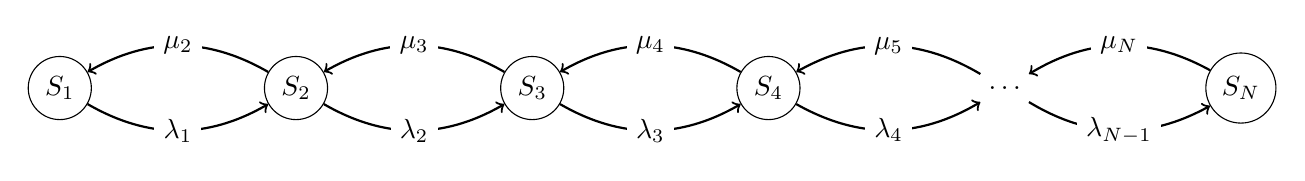
\begin{tikzpicture}
  \begin{scope}[every node/.style={fill=white,circle,draw=black}]
    \node (S_1) at (0,0) {$S_1$};
    \node (S_2) at (3,0) {$S_2$};
    \node (S_3) at (6,0) {$S_3$};
    \node (S_4) at (9,0) {$S_4$};
    \node[draw=white] (S_dots) at (12,0) {$\dots$};
    \node (S_N) at (15,0) {$S_N$};
  \end{scope}

  \begin{scope}[->, every edge/.style={draw=black,thick}, every node/.style={fill=white}]
    \path (S_1) edge [bend right=30] node {$\lambda_1$} (S_2);
    \path (S_2) edge [bend right=30] node {$\mu_2$} (S_1);

    \path (S_2) edge [bend right=30] node {$\lambda_2$} (S_3);
    \path (S_3) edge [bend right=30] node {$\mu_3$} (S_2);

    \path (S_3) edge [bend right=30] node {$\lambda_3$} (S_4);
    \path (S_4) edge [bend right=30] node {$\mu_4$} (S_3);

    \path (S_4) edge [bend right=30] node {$\lambda_4$} (S_dots);
    \path (S_dots) edge [bend right=30] node {$\mu_5$} (S_4);

    \path (S_dots) edge [bend right=30] node {$\lambda_{N-1}$} (S_N);
    \path (S_N) edge [bend right=30] node {$\mu_N$} (S_dots);

    % TODO дописать
  \end{scope}
\end{tikzpicture}

Эта цепь точно является эргодической. Тогда
\[
  \begin{cases}
    0 = -\lambda_1 \pi_1 + \mu_2 \pi_2, \\
    0 = \lambda_1 \pi_1 - (\lambda_2+\mu_2) \pi_2 + \mu_3 \pi_3, \\
    \dots, \\
    0 = \lambda_{N-1} \pi_{N-1} - \mu_N \pi_M, \\
    \sum_j \pi_j = 1.
  \end{cases}
\]

Систему можно решить рекуррентно:
\[
  \begin{cases}
    \pi_2 = \dfrac{\lambda_1}{\mu_2} \pi_1, \\
    \pi_3 = \dfrac{\lambda_2}{\mu_3} \pi_2 = \dfrac{\lambda_2 \lambda_1}{\mu_3 \mu_2} \pi_1, \\
    \ldots, \\
    \pi_N = \dfrac{\lambda_{N-1}}{\mu_N} \pi_{N-1}
    = \ldots
    = \dfrac{\lambda_1 \cdot \ldots \cdot \lambda_{N-1}}{\mu_2 \cdot \ldots
    \cdot \mu_N} \pi_1
    = \dfrac{\prod\limits_{k=1}^{N-1} \lambda_k}{\prod\limits_{j=2}^N \mu_j} \pi_1
    = \prod\limits_{j=2}^N \dfrac{\lambda_{j-1}}{\mu_j} \pi_1,
  \end{cases}
\]
откуда
\[
  \pi_1 = \left( 1 + \sum_{l=2}\prod_{j=2}^N \dfrac{\lambda_{j-1}}{\mu_j} \right)^{-1}.
\]

Если этот ряд сходится (регулярно?), то можно рассматривать и предел
$N \to \infty$, то есть модель, рассматривающую неограниченную популяцию.



\subsection{Системы массового обслуживания}

Системы массового обслуживания обычно обозначаются четвёркой: $(\dots | \dots | \dots | \dots)$,
где в первую записывают закон, по которому поступают <<заказы>>: $M$ -- марковский, % TODO что за марковский
$Er$ -- закон Эрланга,
во вторую записывают закон, по которому мы <<обслуживаем заказы>>: тоже $M$ или $Er$;
в третью -- количество приборов/касс,
в четвертую -- длина очереди (в т.ч. $\infty$).

\begin{figure}[h!]
  \centering
  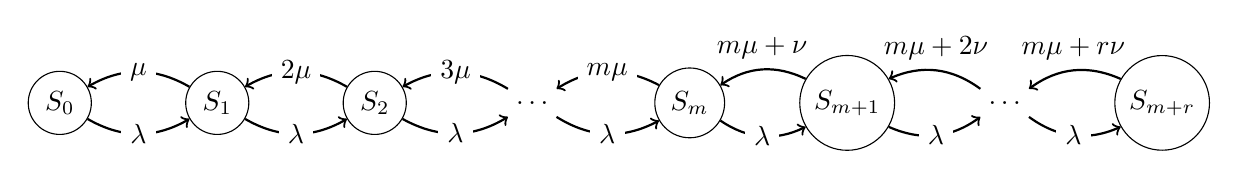
\begin{tikzpicture}
    \begin{scope}[every node/.style={fill=white,circle,draw=black}]
      \node (S_0) at (0,0) {$S_0$};
      \node (S_1) at (2,0) {$S_1$};
      \node (S_2) at (4,0) {$S_2$};
      \node[draw=white] (S_dots_1) at (6,0) {$\dots$};
      \node (S_m) at (8,0) {$S_m$};
      \node (S_{m+1}) at (10,0) {$S_{m+1}$};
      \node[draw=white] (S_dots_2) at (12,0) {$\dots$};
      \node (S_{m+r}) at (14,0) {$S_{m+r}$};
    \end{scope}

    \begin{scope}[->, every edge/.style={draw=black,thick}, every node/.style={fill=white}]
      \path (S_0) edge [bend right=30] node {$\lambda$} (S_1);
      \path (S_1) edge [bend right=30] node {$\lambda$} (S_2);
      \path (S_2) edge [bend right=30] node {$\lambda$} (S_dots_1);
      \path (S_dots_1) edge [bend right=30] node {$\lambda$} (S_m);
      \path (S_m) edge [bend right=30] node {$\lambda$} (S_{m+1});
      \path (S_{m+1}) edge [bend right=30] node {$\lambda$} (S_dots_2);
      \path (S_dots_2) edge [bend right=30] node {$\lambda$} (S_{m+r});

      \path (S_1) edge [bend right=30] node {$\mu$} (S_0);
      \path (S_2) edge [bend right=30] node {$2\mu$} (S_1);
      \path (S_dots_1) edge [bend right=30] node {$3\mu$} (S_2);
      \path (S_m) edge [bend right=30] node {$m\mu$} (S_dots_1);
      \path (S_{m+1}) edge [bend right=30] node[above, fill=none] {$m\mu+\nu$} (S_m);
      \path (S_dots_2) edge [bend right=30] node[above, fill=none] {$m\mu + 2\nu$} (S_{m+1});
      \path (S_{m+r}) edge [bend right=30] node[above, fill=none] {$m\mu + r\nu$} (S_dots_2);
    \end{scope}
  \end{tikzpicture}
\end{figure}

Пусть $\lambda$ -- интенсивность потока заявок, $\mu$ -- интенсивность обслуживания
заявок в пересчёте на прибор, $\nu$ -- интенсивность ухода из очереди.
Состояние $S_i$ -- i приборов занято. $S_{m+j}$ -- $m$ приборов занято и имеется
очередь длины $j$.

Задача решается в стационарном режиме:
\[
  \begin{cases}
    0 = -\lambda \pi_0 + \mu \pi_1, \\
    0 = \lambda \pi_0 - (\lambda+\mu) \pi_1 + 2\mu\pi_2, \\
    \dots \\
    0 = \lambda \pi_{m-1} - (\lambda+m\mu) \pi_m + (m\mu+\nu) \pi_{m+1}, \\
    0 = 
  \end{cases}
  \Rightarrow
  \begin{cases}
    \pi_1 = \dfrac{\lambda}{\mu} \pi_0, \\
    \pi_2 = \dfrac{\lambda}{2\mu}\pi_1 = \dfrac{\lambda^2}{2\mu^2} \pi_0,\\
    \pi_3 = \dfrac{\lambda}{3\mu} \pi_2 = \dfrac{\lambda^3}{3! \cdot \mu^3} \pi_0, \\
    \dots \\
    \pi_m = \dfrac{\lambda^m}{m! \cdot \mu^m} \pi_0, \\
    \pi_{m+1} = \dfrac{\lambda}{m\mu + \nu} \pi_m = \dfrac{\lambda^{m+1}}{m! \cdot \mu^m \cdot (m\mu+\nu)} \pi_0, \\
    \dots\\
    \pi_{m+r} = \dfrac{\lambda^{m+r} \pi_0}{m! \cdot \mu^m \cdot \prod_{k=1}^r (m\mu+k\nu)}
  \end{cases}
\]

Тогда
\[
1 = \pi_0 \left( 1
  + \sum_{j=1}^m \dfrac{\lambda^j}{j! \cdot \mu^j}
+ \dfrac{1}{m!} \sum_{j=m+1}^{m+r} \dfrac{\lambda^j}{\mu^m \prod_{k=1}^j (m\mu + k\nu)} \right).
\]

Обозначим $\alpha = \dfrac{\lambda}{\mu}; \, \beta = \dfrac{\nu}{\mu}$:
\[
  \pi_0 = \left( \sum_{j=0}^m \dfrac{\alpha^j}{j!}
  + \dfrac{1}{m!} \sum_{j=m+1}^{m+r} \dfrac{\alpha^j}{\prod_{k=1}^j (m+k\beta)} \right)^{-1}
\]

\paragraph{Экономические показатели}
\begin{enumerate}
  \item Средняя длина очереди -- математическое ожидание:
    $L = \sum_{k=1}^r k \cdot \pi_{k+m}$

  \item Относительная пропускная способность -- доля обслуженных заявок:
    $q = \dfrac{\lambda - \nu\cdot L}{\lambda}$

  \item Среднее число занятых каналов:
    $K = \sum_{k=0}^m k \pi_k + m \sum_{j=1}^r \pi_{m+j}$.
\end{enumerate}

Соотношения:
\begin{enumerate}
  \item $K = \dfrac{\lambda-\nu L}{\mu} = \alpha - L\beta$.
    По смыслу, $q$ -- доля обслуженных заявок,
    $q\cdot\dfrac{\lambda}{\mu}$ -- число поступивших заявок за время обслуживания одной заявки
    ($\dfrac{1}{\mu}$ -- время обслуживания одной заявки).

  \item $L = \dfrac{\alpha - K}{\beta} = \dfrac{\lambda - \mu K}{\nu}$,
    $q = 1 - \dfrac{\nu}{\lambda} \dfrac{\lambda - \mu K}{\nu} = \dfrac{\mu}{\lambda} K
    = \dfrac{K}{\alpha}$.
\end{enumerate}

\begin{ex}
  Рассматривается СМО (M|M|1|$\infty$) -- 1 обслуживающее устройство, бесконечная очередь.
  Причём рассмотрим случай $\nu = 0$ -- интенсивность ухода из очереди равна нулю.
  \begin{figure}[h!]
    \centering
    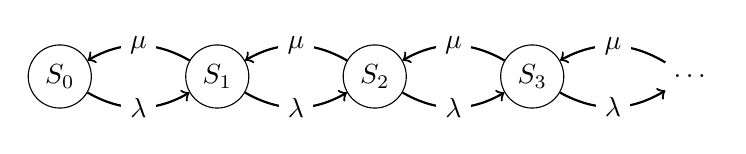
\begin{tikzpicture}
      \begin{scope}[every node/.style={fill=white,circle,draw=black}]
        \node (S_0) at (0,0) {$S_0$};
        \node (S_1) at (2,0) {$S_1$};
        \node (S_2) at (4,0) {$S_2$};
        \node (S_3) at (6,0) {$S_3$};
        \node[draw=white] (S_dots) at (8,0) {$\dots$};
      \end{scope}
    
      \begin{scope}[->, every edge/.style={draw=black,thick}, every node/.style={fill=white}]
        \path (S_0) edge [bend right=30] node {$\lambda$} (S_1);
        \path (S_1) edge [bend right=30] node {$\lambda$} (S_2);
        \path (S_2) edge [bend right=30] node {$\lambda$} (S_3);
        \path (S_3) edge [bend right=30] node {$\lambda$} (S_dots);

        \path (S_dots) edge [bend right=30] node {$\mu$} (S_3);
        \path (S_3) edge [bend right=30] node {$\mu$} (S_2);
        \path (S_2) edge [bend right=30] node {$\mu$} (S_1);
        \path (S_1) edge [bend right=30] node {$\mu$} (S_0);
      \end{scope}
    \end{tikzpicture}
  \end{figure}
  \[
    \begin{cases}
      0 = -\lambda \pi_0 + \mu \pi_1, \\
      0 = \lambda \pi_0 - (\lambda+\mu) \pi_1 + \mu \pi_2, \\
      \dots\\
      0 = \lambda \pi_{k-1} - (\lambda+\mu) \pi_k + \mu \pi_{k+1}, \\
      \dots
    \end{cases}
    \Rightarrow
    \begin{cases}
      \pi_1 = \dfrac{\lambda}{\mu} \pi_0, \\
      \pi_2 = \dfrac{\lambda}{\mu}\pi_1 = \dfrac{\lambda^2}{\mu^2} \pi_0, \\
      \dots \\
      \pi_k = \left( \dfrac{\lambda}{\mu} \right)^k \pi_0.
    \end{cases}
  \]
  \[
    \pi_0 \sum_{k=0}^\infty \alpha^k = 1 \Rightarrow \pi_0 = 1 - \alpha.
  \]
  -- этот ряд сходится при $\alpha < 1$.

  Средняя длина очереди:
  \[
    L = \sum_{k=1}^\infty k \cdot \pi_{k+1}
    = \sum_{k=1}^\infty k\cdot \alpha^{k+1} (1-\alpha)
    = \alpha^2 (1-\alpha) \sum_{k=1}^\infty k \alpha^{k+1}
     = \alpha^2 (1-\alpha) \left( \dfrac{1}{1-\alpha} \right)' = \dfrac{\alpha^2}{1-\alpha}
  \]
\end{ex}

\paragraph{Закон распределения времени ожидания (от себя)}
В условиях этого примера рассмотрим закон распределения времени ожидания.
Обозначим время ожидания $T$. В простейшем случае заказ приходит, когда
очередь пустая и обслуживающее устройство простаивает, в этом случае:
$P(T = 0) = \pi_0 = 1-\alpha$. Рассмотрим функцию
$f(t) = P(T > t) = \sum_{i=1}^\infty \pi_i \cdot \hat{p}_i (t)$:
когда заказ приходит в очереди уже есть $i$ заказов с вероятностью $\pi_i$.
$\hat{p}_i(t)$ -- %вероятность события $(T > t)$ в марковской цепи:
закон распределения времени пребывания в такой марковской цепи: 
\begin{figure}[h!]
  \centering
  \begin{tikzpicture}
    \begin{scope}[every node/.style={fill=white,circle,draw=black}]
      \node (S_0) at (0,0) {$S_0$};
      \node (S_1) at (2,0) {$S_1$};
      \node (S_2) at (4,0) {$S_2$};
      \node[draw=white] (S_dots) at (6,0) {$\dots$};
      \node (S_i) at (8,0) {$S_i$};
    \end{scope}
  
    \begin{scope}[->, every edge/.style={draw=black,thick}, every node/.style={fill=white}]
      \path (S_i) edge node {$\mu$} (S_dots);
      \path (S_dots) edge node {$\mu$} (S_2);
      \path (S_2) edge node {$\mu$} (S_1);
      \path (S_1) edge node {$\mu$} (S_0);
    \end{scope}
    \node[draw=black,very thick,dotted,fit=(S_1) (S_i)] (FIt1) [acateur][label=above:{$U$}]{};
  \end{tikzpicture}
\end{figure}

То есть нас не интересует очередь после прихода заказа, за которым мы следим.
Для этой цепи быстренько находим закон распределения времени нахождения в
подмножестве состояний $U$:
\[
  \begin{cases}
    p_i'=-\mu p_i,\\
    p_{i-1}'=\mu p_i - \mu p_{i-1},\\
    \dots\\
    p_{i-k}' = \mu p_{i-k+1} - \mu p_{i-k},\\
    \dots\\
    p_0' = \mu p_1,
  \end{cases}
  \Rightarrow
  \begin{cases}
    s \tilde{p}_i-1 = -\mu \tilde{p}_i, \\
    s \tilde{p}_{i-1} = \mu \tilde{p}_i - \mu \tilde{p}_{i-1},\\
    \dots\\
    s \tilde{p}_{i-k} = \mu \tilde{p}_{i-k+1} - \mu \tilde{p}_{i-k},\\
    \dots\\
    s\tilde{p}_0 = \mu \tilde{p}_1
  \end{cases}
  \Rightarrow
  \begin{cases}
    \tilde{p}_i = \dfrac{1}{s+\mu},\\
    \tilde{p}_{i-1} = \dfrac{\mu}{s+\mu} \tilde{p}_i = \dfrac{\mu}{(s+\mu)^2}, \\
    \dots\\
    \tilde{p}_{i-k} = \dfrac{\mu^k}{(s+\mu)^{k+1}}, \\
    \dots\\
    \tilde{p}_0 = \dfrac{\mu^i}{s (s+\mu)^i} 
  \end{cases}
\]
Обратное преобразование выполним с помощью теоремы разложения:
две степенных особенности в точках $0$ и $-\mu$:
\begin{multline*}
  \tilde{p}_0 \risingdotseq \lim_{s\to 0} \dfrac{\mu^i}{\mu^i} e^{st} 
  + \dfrac{\mu^i}{(i-1)!} \lim_{s\to -\mu} \dfrac{d^{i-1}}{ds^{i-1}} \left( \dfrac{1}{s} \cdot e^{st} \right)
  = 1
  + \dfrac{\mu^i}{(i-1)!} \sum_{j=0}^{i-1} C_{i-1}^j \lim_{s\to -\mu}
  \left( \dfrac{d^j (1/s)}{ds^j} \cdot \dfrac{d^{i-j-1} e^{st}}{ds^{i-j-1}} \right) = \\
  = 1 + \dfrac{\mu^i}{(i-1)!} \sum_{j=0}^{i-1} C_{i-1}^j \lim_{s\to -\mu} \left(
  (-1)^j \dfrac{j!}{s^{j+1}} \cdot t^{i-j-1} e^{st} \right)
  = 1 + e^{-\mu t} \sum_{j=0}^{i-1} \dfrac{(\mu t)^{i-j-1}}{(i-j-1)!}
  = 1 - \dfrac{\Gamma_{\mu t}(i)}{\Gamma(i)},
\end{multline*}
где $\Gamma_{\mu t}(i) = \int_{0}^{\mu t} x^{i-1} \cdot e^{-x} \, dx$ -- неполная
гамма-функция. Тогда закон распределения времени пребывания в подмножестве $U$:
\[
  \hat{p}_i (t) = 1 - p_0(t) = \dfrac{\Gamma_{\mu t} (i)}{\Gamma(i)}.
\]
Подставим это в сумму и поменяем знаки интегрирования и суммирования
(учитывая равномерную и абсолютную сходимость ряда):
\begin{multline*}
  f(t) = P(T>t) = \sum_{i=1}^\infty \pi_i \cdot \dfrac{\Gamma_{\mu t} (i)}{\Gamma(i)}
  = (1-\alpha) \int\limits_0^{\mu t} \sum_{i=1}^\infty \dfrac{\alpha^i}{(i-1)!} x^{i-1} \cdot e^{-x} \, dx = \\
  = (1-\alpha) \alpha \int\limits_0^{\mu t} e^{-x} \sum_{k=0}^\infty \dfrac{(\alpha x)^k}{k!} \, dx
  = (1-\alpha) \alpha \int\limits_0^{\mu t} e^{-(1-\alpha)x} \, dx
  = \alpha \left( e^{0} - e^{-(1-\alpha)\mu t} \right) = \\
  = \alpha \left( 1 - e^{- (\mu - \lambda) t} \right) 
\end{multline*}

% TODO
Ответ получился неправильный, правильный ответ:
$f(t) = P(T > t) = \alpha e^{-(\mu - \lambda) t}$.

